\section{NP-kompletheds Beviser}%
\label{sec:npkomplethed}

\begin{frame}
	\frametitle{Pensum}
	\begin{itemize}
		\item Siper 7.1-7.4: \textbf{Tidskompleksitet inkl. P, NP, NP-komplethed}
		\item CLRS 34: \textbf{NP-Komplethed Beviser} (minus sider 1070-1078)
		\item Weekly Note 7
		\item Weekly Note 8
		\item Weekly Note 9 (ish)
		\item Video 15-17
	\end{itemize}
\end{frame}

\subsection{Måling af kompleksitet}%
\label{subsec:label}

\begin{frame}[allowframebreaks]
	\frametitle{Kompleksitet}
	\begin{itemize}
		\item Trods der eksisterer sprog som vi kan afgøre i teori, kan vi ofte ikke afgøre dem \textit{i praksis}, grundet deres kompleksitet (køretid.)
		\item Vi vil kigge på sproget $A = \{0^{k}1^{k} \mid k \ge 0\}$.
		\item Vi laver en algoritme, og finder dens køretid.
		\item $M_{1} = $''På input streng $w$:
		      \begin{enumerate}
			      \item Scan henover båndet og \textit{afvis} hvis et 0 findes til højre af et 1. (Altså hvis den ser et 1, og så et 0).
			      \item Gentag hvis der stadig er 0 og 1 på båndet:
			            \begin{enumerate}
				            \item Scan henover båndet og afkryds hvert 0 og hvert 1
			            \end{enumerate}

			      \item Hvis der stadig er 0'er tilbage efter 1 er blevet krydset af, eller omvendt, så \textit{afvis}. Ellers \textit{accepter}.
		      \end{enumerate}

		\item Køretiden af en algoritme kan være afhængig af flere parametre.
		\item Hvis algoritmen kører på en graf, kan den for eksempel være afhængig af antallet af knuder og kanter.
		\item I \textit{worst-case køretid} kigger vi på hvad det værst mulige tilfælde er, givet alle inputs af en længde (ofte $n$).
	\end{itemize}
	\begin{definition}
		Lad $M$ være en deterministisk TM som standser på alle input. \textit{Køretiden} eller \textit{tidskompleksiteten} af $M$ er funktionen $f : \mathcal{N} \rightarrow \mathcal{N}$, hvor $f(n)$ er maksimumsantallet af skridt som $M$ tager på et input af længde $n$. Hvis $f(n)$ er køretiden af $M$, så siger vi at $M$ kører i tid $f(n)$ og at $M$ er en $f(n)$-tids Turingmaskine. Vi bruger normalvis $n$ til at repræsentere længden af et input.
	\end{definition}
\end{frame}

\begin{frame}[allowframebreaks]
	\frametitle{Store-O og lille-O notation}
	\begin{itemize}
		\item Den præcise køretid af en algoritme er ofte meget kompleks.
		\item Derfor bruger vi \textit{asymptotisk analyse}.
		\item Ved asymptotisk notation kigger vi ikke på koefficienter og kun ``highest order term'' af udtrykket af køretiden. Så for eksempel bliver $2n+3$ bare til $n$.
		\item Et andet eksempel er $f(n) = 6n^{3} + 2n^{2}+20n+45$. Dette bliver til $f(n) = O(n^{3})$.
		\item Asymptotisk notation er også det der kalders store-$O$ notation.
	\end{itemize}

	\begin{definition}
		Lad $f$ og $g$ være funktioner $f,g : \mathcal{N} \rightarrow \mathcal{R}^{+}$. Vi siger at $f(n) = O(g(n))$ hvis positive heltal $c$ og $n_{o}$ eksisterer således at for hvert heltal $n \ge n_{0}$,
		\begin{equation}
			f(n) \le cg(n)
		\end{equation}
		Når $f(n) = O(g(n))$, siger vi at $g(n)$ er et \textit{upper bound}, eller \textit{øvre grænse} for $f(n)$, eller mere præcist at $g(n)$ er en asymptotisk øvre grænse for $f(n)$.
	\end{definition}
	\begin{itemize}
		\item Intuitivt betyder $f(n) = O(g(n))$ at $f$ er mindre end eller lig med $g$.
		\item Bemærk også her at logaritmens base er undertrykket, så $\log_{2}$ bliver bare til $O(\log)$
		\item Det vil altså sige at $f_{2}(n) = 3n \log_{2} n + 5n \log_{2}\log_{2}n+2 = O(n \log n)$.
		\item Store-$O$ kan også findes i arimetiske udtryk såsom $f(n) = O(n^{2})+O(n)$ bemærk dog at dette blot er lig med $O(n^{2})$ da $n^{2} > n$.
		\item Ved $f(n) = 2^{O(n)}$ er dette et udtryk for $2^{cn}$, for en konstant $c$.
		\item Lille-$o$ notation siger at en funktion er asymptotisk mindre end en anden.
		\item Analogt til store-$O$ og lille-$O$ er hhv. $\le$ og $<$.
	\end{itemize}

	\begin{definition}
		Lad $f$ og $g$ være funktionerne $f, g : \mathcal{N} \rightarrow \mathcal{R}^{+}$. Say that $f(n) = o(g(n))$ hvis
		\begin{equation*}
			\lim_{n \rightarrow \infty} \frac{f(n)}{g(n)} = 0
		\end{equation*}
		I andre ord betyder $f(n) = o(g(n))$ at for alle reelle tal $c > 0$, eksisterer der et tal $n_{0}$ hvor $f(n) < cg(n)$ for alle $n \ge n_{0}$
	\end{definition}

	\begin{itemize}
		\item Følgende er eksempler af ligninger med lille-$o$:
		\item $\sqrt{n} = o(n)$
		\item $n = o(n \log \log n)$
		\item $n \log \log n = o(n \log n)$
		\item $n \log n = o(n^{2})$
		\item $n^{2} = o(n^{3})$
	\end{itemize}
\end{frame}

\begin{frame}[allowframebreaks]
	\frametitle{Analyse af Algoritmer}
	\begin{itemize}
		\item Nu vil vi faktisk til at analysere algoritmen vi konstruerede tidligere.
		\item $M_{1} = $''På input streng $w$:
		      \begin{enumerate}
			      \item Scan henover båndet og \textit{afvis} hvis et 0 findes til højre af et 1. (Altså hvis den ser et 1, og så et 0).
			      \item Gentag hvis der stadig er 0 og 1 på båndet:
			            \begin{enumerate}
				            \item Scan henover båndet og afkryds hvert 0 og hvert 1
			            \end{enumerate}

			      \item Hvis der stadig er 0'er tilbage efter 1 er blevet krydset af, eller omvendt, så \textit{afvis}. Ellers \textit{accepter}.
		      \end{enumerate}

		\item Vi analysere hver af dens fire stadier seperat.
		      \begin{enumerate}
			      \item At scanne tager $n$ skridt, da længden af strengen er $n$. Vi skal også tilbage igen, og dette tager $n$ skridt. I alt $2n$. (Husk at $2n = O(n)$)
			      \item[2-3] Hvert scan her bruger $O(n)$ skridt. Fordi hver scan afkrydser to symboler, er det højets $n/2$ scanninger (fordi vi krydser to af hver gang.) Dermed er tiden taget af stadier 2-3 $(n/2)O(n) = O(n^{2})$ skridt.
			      \item[4] Tiden den bruger på at finde ud af dette er \textit{højest} $O(n)$.
		      \end{enumerate}
		\item Dermed er tiden $O(n) + O(n^{2})+O(n) = O(n^{2})$
	\end{itemize}

	\begin{definition}
		Lad $t : \mathcal{N} \rightarrow \mathcal{R}^{+}$ være en funktion. Vi definerer \textit{tidskompleksitetsklassen} $TIME(t(n))$ til at være samlingen af alle sprog der er afgjort af en Turingmaskine som kører i $O(t(n))$ tid.
	\end{definition}
	\begin{itemize}
		\item Det vil altså sige at algoritmen $A$ vi analyserede før er en del af $TIME(n^{2})$, altså $A \in TIME(n^{2})$.
		\item Jeg har udeladt et bevis for at denne algoritme kan afgøres i $O(n \log n)$ tid, men en vigtigt takeaway fra dette er at alle sprog der kan afgøres i $o(n \log n)$ (bemærk lille-$o$!) er regulære.
		\item Church-turing tesen (som er beregnelighedsteori) siger at alle ``reasonable'' modeller af komputering er ækvivalente.
		\item I kompleksitetsteori bestemmer modelvalget kompleksiteten på et sprog.
		\item For eksempel kan $A$ afgøres i $O(n)$ tid på en 2-bånds Turingmaskine.
	\end{itemize}
\end{frame}

\begin{frame}[allowframebreaks]
	\frametitle{Kompleksitetsforholdet mellem modeller}

	\begin{itemize}
		\item Vi vil nu kigge på hvordan valget af en model kan påvirke køretiden af sprog.
		\item Vi kigger på tre modeller: enkeltbåndsmaskinen, multibåndsmaskionen og den nondeterministiske maskine.
	\end{itemize}

	\begin{theorem}
		Lad $t(n)$ være en funktion hvor $t(n) \ge n$. Så for hver $t(n)$-tids multibånds Turingmaskine, er der en ækvivalent $O(t^{2}(n))$-tids enkelt-bånds Turingmaskine.
	\end{theorem}
	\begin{itemize}
		\item Vi vil vise dette ved at analysere algoritmen vi brugte tidligere til at konvertere fra multibånds til enkeltbånds.
		\item Lad $M$ være en $k$-bånds TM der kører i $t(n)$ tid.
		\item Lad $S$ være en enkeltbånds TM der kører i $O(t^{2}(n))$ tid.
		\item $S$ simulerer $M$ som beskrevet (meget) tidligere.
		\item Til at starte med tager $S$ sit bånd i det format der repræsenterer alle bånd af $M$ og simulerer derefter $M$'s skridt.
		\item For at simulere et skridt scanner $S$ al informationen for at bestemme informationerne under symbolerne ved $M$'s båndhoveder.
		\item $S$ laver så en til scanning over dets bånd til at opdatere båndindholdet og hovedpositioner.
		\item Hvis en af hovederne går til højre mere end der er plads til, rightshifter vi.
		\item For hvert skridt af $M$, laver $S$ to scanninger over den aktive del af dens bånd. Den første scanning får informationen nødvendigt til at bevæge sig, og den anden scanning udfører denne bevægelse.
		\item Hvert bånd i $M$ har længde højest $t(n)$, da det er muligt at hovedet bevæger sig til højre for hvert skridt.
		\item Dermed bruger en scanning af den aktive del af $S$' bånd højest $O(t(n))$ skridt.
		\item For at simulerer hvert af $M$'s skridt, laver $S$ to scanninger og op til $k$  højreshifts, hver bruger $O(t(n))$ tid, så den endelige tid til ét skridt et $O(t(n))$.
		\item Vi sætter nu en grænse på den endelige tid af hele $S$:
		      \begin{enumerate}
			      \item Først tager 4S båndet i den rigtige format. Dette bruger $O(n)$ tid.
			      \item Så simulerer $S$ hvert af de $t(n)$ skridt af $M$, dette bruger $O(t(n))$ tid. Denne del af simuleringen bruger altså $t(n) \times O(t(n)) = O(t^{2}(n))$ trin.
			      \item Dermed er hele simuleringen $O(n) + O(t^{2}(n))$ skridt.
			      \item $O(n) + O(t^{2}(n)) = O(t^{2}(n))$
		      \end{enumerate}

		\item Vi vil nu kigge på nondeterministisk Turingmaskines køretid og en simulerende køretid.
	\end{itemize}
	\begin{definition}
		Lad $N$ være en NDTM som er afgører. \textit{Køretiden} af $N$ er funktionen $f : \mathcal{N} \rightarrow \mathcal{N}$, hvor $f(n)$ er det maksimum antal af skridt som $N$ bruger på en gren af dens komputering, på en længde $n$.
	\end{definition}

	\begin{center}
		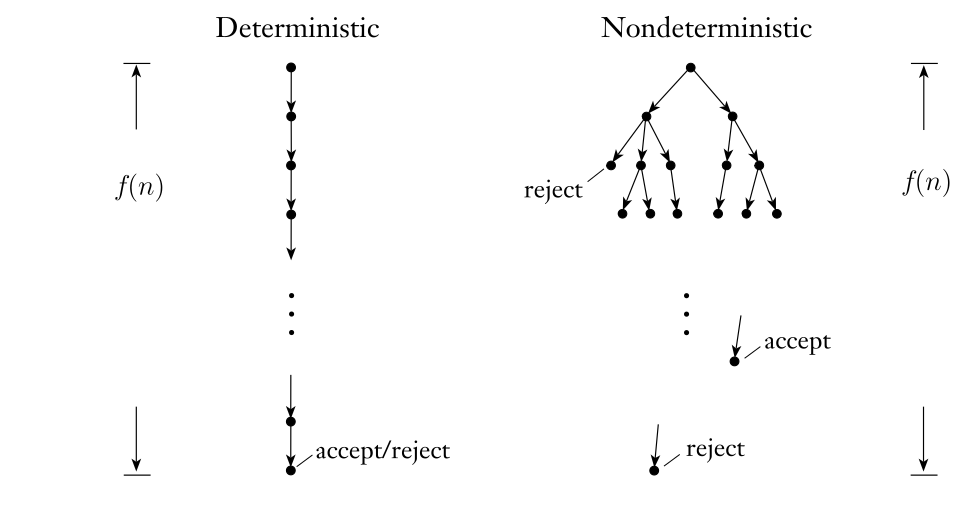
\includegraphics[scale=0.3]{figur/figur710.png}
	\end{center}

	\begin{theorem}
		Lad $t(n)$ være en funktion, hvor $t(n) \ge n$. Så for hver $t(n)$ tids NDTM enkeltbånds Turingmaskine, har den ækvivalent $2^{O(t(n))}$-tids (D)TM på et enkelt bånd.
	\end{theorem}

	\begin{itemize}
		\item På en input længde $n$, så har hver gren af $N$'s træ længde højest $t(n)$.
		\item Hver knude i træet har højest $b$ børn, hvor $b$ er det maskimale antal af lovlige valg af $N$'s overføringsfunktion.'s overføringsfunktion.
		\item Dermed er det endelige antal af blade i træet højest $b^{t(n)}$
		\item Simuleringerne går videre ved at udforske træet i BFS.
		\item Antallet af knuder i træet er mindre end det dobbelte af antallet af blade, så vi kan sætte en grænse $O(b^{t(n)})$.
		\item Tiden det tager at gå fra roden til en knude er $O(t(n))$.
		\item Køretiden er altså $O(t(n)b^{t(n)}) = 2^{O(t(n))}$.
	\end{itemize}
\end{frame}

\subsection{Klassen $P$}%
\label{subsec:label}

\begin{frame}[allowframebreaks]
	\frametitle{Klassen $P$}
	\begin{itemize}
		\item Vi så tidligere at en multibånds TM kan konverteres til en enkeltbånds TM der kører i $O(n^{2})$ tid, altså polynomiel.
		\item Vi så også at en NDTM kan konverteres til en TM der kører i $2^{O(n)}$ tid, som altså er eksponentielt.
		\item Vi differentierer ofte algoritmer mellem at være \textit{eksponentielle} og \textit{polynomielle}, hvor vi synes at de polynomielle algoritmer er en del hurtigere end de eksponentielle.
		\item For eksempel polynomiet $n^{3}$ og eksponenten $2^{n}$. Hvis $n = 1000$ så er $n^{3} \approx 1 000 000 000$, hvorimod $2^{n}$ er langt større end antallet af atomer i universet (mellem $10^{78}$ og $10^{82}$).
		\item Vi får ofte eksponentielle algoritmer ved at lave brute-force løsninger til problemer.
	\end{itemize}

	\begin{definition}
		$P$ er klassen af sprog som af afgørlige i polynomiel tid på en deterministisk enkeltbånds Turingmaskine.
		\begin{equation}
			P = \bigcup_k TIME(n^{k})
		\end{equation}
	\end{definition}

	\begin{itemize}
		\item Klassen $P$ er vigtig fordi:
		      \begin{enumerate}
			      \item $P$ er en invariant for alle modeller der er polynomielt ækvivalente til en enkeltbånds TM
			      \item $P$ er nogenlunde det vi tænker på som klassen af problemer vi realistisk set kan løse på en computer
		      \end{enumerate}
	\end{itemize}
\end{frame}

\begin{frame}[allowframebreaks]
	\frametitle{Eksempler på problemer i $P$}
	\begin{itemize}
		\item Når vi repræsenterer problemerne i kodning (\(\langle M \rangle\)), antager vi at denne kodning er rimelig, og kan blive sat om til en intern repræsentation i polynomiel tid.
		\item Vi vil i disse eksempler kigge meget på grafer.
		\item En rimelig kodning af en graf er en liste af dens knuder og kenter.
		\item En anden rimelig kodning (som også oftest er brugt i programmering) er en \textit{adjacency matrix}, hvor den $(i,j)$'e ``entry'' er $1$ hvis der er en kant fra knude $i$ til knude $j$, og 0 ellers.
		\item Det første problem omhandler rettede grafer, nemlig $PATH$ problemet.
	\end{itemize}

	\begin{equation}
		PATH = \{\langle G, s, t \rangle \mid G \text{ er en rettet graf med en rettet vej fra } s \text{ til } t\}
	\end{equation}

	\begin{theorem}
		$PATH \in P$
	\end{theorem}

	\begin{itemize}
		\item Vi beviser ved at konstruere en algoritme der kører i polynomiel tid. Først kigger vi dog på brute-force løsningen, som vi kan konkludere ikke er hurtig nok.
		\item En Brute-force løsning kigger alle mulige veje og tjekker om nogen af dem er rettet fra $s$ til $t$.
		\item En vej kan længst have længde $m$ hvor $m$ er antallet af knuder. ($m$ fordi det aldrig vil være nødvendigt at gentage en knude.)
		\item Antallet af potentielle veje er cirka $m^{m}$, som er eksponentielt baseret på antal knuder i $G$.
		\item Altså er brute-force algoritmen $\notin P$.
		\item Hvis vi i stedet kører en form for BFS får vi en algoritme der kører i polynomiel tid:
		\item $M =$''På input \(\langle G, s, t \rangle \) hvor $G$ er en rettet graf med knuder $s$ og $t$.
		      \begin{enumerate}
			      \item Markér knude $s$
			      \item Gentag følgende indtil der ikke er flere knuder der bliver markeret:
			            \begin{enumerate}
				            \item Scan alle knuder af $G$. Hvis en kant $(a,b)$ er fundet ved at gå fra en markeret knude $a$ til en markeret knude $b$, markér knude $b$.
			            \end{enumerate}
			      \item Hvis $t$ er markeret, \textit{accepter} og ellers \textit{afvis}.
		      \end{enumerate}
		\item Hvis $t$ markeres er der fundet en vej fra $s$ til $t$.
		\item Stadierne 1 og 3 kører kun en enkelt gang.
		\item Stadie 2 kører højest $m$ gange, fordi hver gang tager den en til knude.
		\item Dermed er antallet af stadier brugt højest $m+2$, hvilket er polynomielt i $G$.
		\item Vi kigger nu på problemet om \textit{relative primtal} (også kaldet inbyrdisk primiske).
		\item To tal er indbyrdisk primiske hvis 1 er det største heltal som ligeligt deler dem begge.
		\item For eksempel er 10 og 21 indbyrdisk primiske, selvom ingen af dem er primtal. 10 og 22 er dog ikke indbyrdisk primiske fordi begge er delelige med $2$.
		\item Vi definerer nu problemet $RELPRIME$.
	\end{itemize}

	\begin{equation}
		RELPRIME = \{\langle x, y \rangle \mid x \text{ og } y \text{ er indbyrdisk primiske}\}
	\end{equation}

	\begin{theorem}
		$RELPRIME \in P$
	\end{theorem}

	\begin{itemize}
		\item En måde at løse dette på er ved at gå alle tal igennem, og se om de er delelige med tallene. Dette er dog eksponentielt i sin køretid.
		\item I stedet bruger vi Euklids algoritme, som vi havde om i Diskret Matematik.
		\item Denne kører polynomielt.
		\item Følgende er Euklids algoritme:
		\item $E = $''På input \(\langle x,y\rangle\), hvor $x$ og $y$ er naturlige tal i binær:
		      \begin{enumerate}
			      \item Gentag indtil $y = 0$:
			            \begin{enumerate}
				            \item[2] $x \leftarrow x \mod y$
				            \item[3] Byt $x$ og $y$
			            \end{enumerate}
			      \item[4] Output $x$''
		      \end{enumerate}
		\item Vi bruger $E$  som subrutine i algoritmen $R$:
		\item $R = $''På input \(\langle x, y \rangle\), hvor $x$ og $y$ er naturlige tal i binær:
		      \begin{enumerate}
			      \item Kør $E$ på \(\langle x, y \rangle \)
			      \item Hvis resultatet er $1$, \textit{accepter}, ellers \textit{afvis}.''
		      \end{enumerate}

		\item Vi vil nu vise at $E$ og dermed $R$ er polynomielt.
		\item Stadie 2 af $R$ skærer værdien mindst halvt.
		\item Efter stadie 2, er $x < y$.
		\item Efter stadie 3 er $x > y$, da vi har byttet værdierne.
		\item Når stadie 2 eksekveres er $x > y$.
		\item Hvis $x/2 < y$, så $x \mod y = x - y < x / 2$, og $x$ ryger mindst ned til halvdelen
		\item De originale værdier af $x$ og $y$ byttes hver gang stadie 3 kører.
		\item Dermed er maksimums antallet af gangene stadie 2 og 3 køres den $\min\{ 2 \log_{2} x, 2 \log_{2} y\}$
		\item Disse logaritmer er propertionelle til længderne af repræsentationerne.
		\item Hvert stadie i $E$ bruger polynomiel tid, og da antallet af stadier der køres er $O(n)$ er den endelige køretid polynomiel.
		\item Sidst kigger vi på problemet om at alle kontekstfrie sprog er afgørlige i polynomiel tid.
	\end{itemize}

	\begin{theorem}
		Hvert kontekstfrit sprog $\in P$.
	\end{theorem}

	\begin{itemize}
		\item Algoritmen vi konstruerede tidligere til at bevise at alle kontekstfrie sprog var afgørlige er \textbf{ikke} nok her!
		\item Den algoritme forsøger alle afledninger med $2n-1$ skridt, når dens input er en streng af længde 4n.
		\item Antallet af afledninger med $k$ skridt kan være eksponentielt i $k$.
		\item For at få en algoritme der kører i polynomiel tid bruger vi \textit{dynamic programming}.
		\item Dynamic programming holder på løsningsinformation og deler problemer op i mindre problemer.
		\item Vi gør dette ved at lave en table af alle delproblemer, og putter deres løsninger ind systematisk, som vi finder dem.
		\item I det her tilfælde er delproblemerne om hver variabel i $G$ genererer hver delstreng i $w$.
		\item Algoritmen putter løsningen ind i en tabel af størrelse $n \times n$.
		\item Hvor $i \le j$, er den $(i,j)$'e ``entry'' i tabellen samlingen af variabler der genererer delstringen $w_{i}w_{i+1}\ldots w_{j}$. Hvor $i > j$ er ``entriesne'' ikke brugt.
		\item Algoritmen fylder hver entry for hver delstreng af $w$.
		\item Først fylder den for delstrengene af længde 1, så længde 2, etc.
		\item Den bruger disse entries til de mindre længder til at hjælpe med at bestemme entries i længere længder.
		\item Antag for eksempel at algoritmen allerede har fundet ud af hvilke variabler genererer alle delstrenge op til længde $k$.
		\item For at bestemme om en variabel $A$ genererer to delstrenge af længde $k+1$, splitter algoritmen edn delstreng i to dele på de $k$ mulige måder.
		\item For hvert split, kigger algoritmen på reglen $A \rightarrow BC$, for at bestemmet om $B$ genererer den første del og $C$ den anden del.
		\item Hvis både $B$ og $C$ genererer hhv. første og anden del, så genererer $A$ delstrengen og kan blive tilføjet til tabellen.
		\item Algoritmen starter processen med strenge af længde $1$ ved at kigge efter regler $A \rightarrow b$
		\item Den følgende algoritme implementerer idéen præsenteret tidligere.
		\item Lad $G$ være en Chomsky grammatik der genererer CFL'et $L$.
		\item Antag at $S$ er startvariablen.
	\end{itemize}
	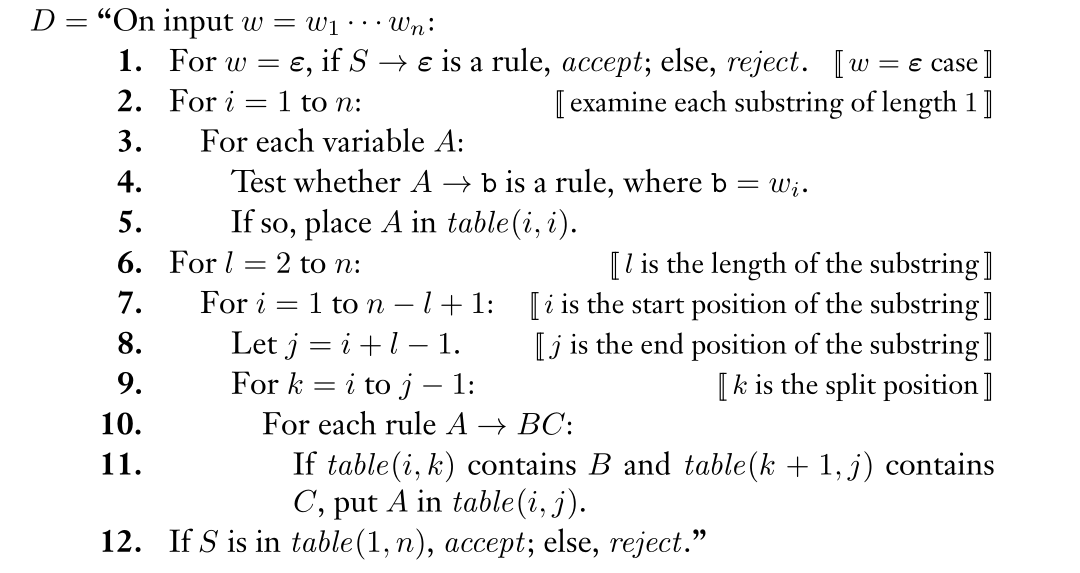
\includegraphics[scale=0.3]{figur/polycfg.png}
	\begin{itemize}
		\item Stadierne $4$ og $5$ kører højest $nv$ gange, hvor $v$ er antallet af variabler.
		\item Disse stadier kører altså $O(n)$ gange
		\item Stadie 6 kører højest $n$ gange.
		\item Hver gang stadie 6 kører, kører stadie 7 højest $n$ gange.
		\item Hver gang stadie 7 kører, kører stadierne 8 og 9 højest $n$ gange.
		\item Hver gang stadie 9 kører, kører stadie 10 $r$ gange, hvor $r$ er antallet af regler
		\item Stadie 3, den indre løkke, kører $O(n^{3})$ gange.
		\item $O(n) + O(n) + \ldots + O(r) + O(n^{3}) = O(n^{3})$
	\end{itemize}
\end{frame}

\subsection{Klassen $NP$}%
\label{subsec:label}

\begin{frame}[allowframebreaks]
	\frametitle{Klassen $NP$}
	\begin{itemize}
		\item Nogen problemer kender vi ikke polynomielle løsninger til.
		\item Et eksempel på et sådan problem er $HAMPATH$ problemet.
	\end{itemize}

	\begin{align*}
		HAMPATH = & \{\langle G, s, t \rangle \mid G \text{ er en rettet graf med en HAMPTH fra } \\
		          & s \text{ til } t\}
	\end{align*}

	\begin{itemize}
		\item En hamiltoniansk vej er en rettet vej som går gennem hver knude én gang.
		\item Trods der ikke eksisterer en polynomiel løsning til Hampath problemet, kan vi verificere løsningen i polynomiel tid.
		\item Altså kan vi overbevises om at en løsning til problemet er en korrekt løsning i polynomiel tid.
	\end{itemize}

	\begin{definition}
		En \textit{verifikator} for et sprog $A$ er en algoritme $V$, hvor
		\begin{equation*}
			A = \{w \mid V \text{ accepterer } \langle w, c \rangle \text{ for en streng }c\}
		\end{equation*}

		Vi regner tiden for en verifikator kun ud fra længden af $w$, så en verifikator i polynomiel tid kører i polynomiel tid i længden af $w$. Et sprog $A$ er verificerbart i polynomiel tid hvis det har en verifikator der kører i polynomiel tid.
	\end{definition}

	\begin{itemize}
		\item $c$ kaldes for et \textit{certifikat} eller \textit{bevis} af medlemskab i $A$.
		\item For verifikatorerer i polynomiel tid, har certifikatet også polynomiel længde i $w$, fordi det er alt verifikatoren kan nå.
		\item For eksempel, ved HAMPATH problemet er et certifikat en vej fra $s$ til $t$.
		\item
	\end{itemize}
	\begin{definition}
		$NP$ er klassen af sprog som har verifikatorer i polynomiel tid.
	\end{definition}
	\begin{itemize}
		\item Denne definition klargører også at $P \subseteq NP$.
		\item Følgende er en NDTM der afgører HAMPATH problemet i polynomiel tid:
		\item $N_{1} = $''På input \(\langle G, s, t \rangle\), hvor $G$ er en rettet graf med knuder $s$ og $t$:
		      \begin{enumerate}
			      \item Skriv en liste af $m$ tal $p_{1}, \ldots, p_{m}$, hvor $m$ er antallet af knuder i $G$. Hver tal i listen er nondeterministisk valgt til at være mellem $1$ og $m$.
			      \item Se om der er nogle ens tal, hvis der er \textit{afvis}
			      \item Tjek om $s = p_{1}$ og $t = p_{m}$. Hvis ikke \textit{afvis}.
			      \item For hvert $i$ mellem $1$ og $m-1$, tjek om $(p_{i}, p_{i+1})$ er en kant i $G$. Hvis ikke, \textit{afvis}. Ellers \textit{accepter}.
		      \end{enumerate}
	\end{itemize}

	\begin{theorem}
		Et sprog $A$ er i $NP$ $\iff$ $A$ er afgjort  af en NDTM i polynomiel tid.
	\end{theorem}

	\begin{itemize}
		\item Vi viser hvordan man konverterer en verifikator i polynomiel tid, til en NDTM i polynomiel tid, og omvendt.
		\item NDTM'en simulerer verifikatoren ved at gætte på certifikatet.
		\item Verifikatoren simulerer NDTM'en ved at bruge den accepterende gren som certifikat.
		\item \(\Rightarrow\) Lad $A \in NP$. Lad $V$ være vertifikatoren i polynomiel tid for $A$. Antag at $V$ er en Turingmaskine der kører i tid $n^{k}$ og konstruer $N$:
		\item $N =$''På input $w$ af længde $n$:
		      \begin{enumerate}
			      \item Nondeterministisk vælg streng $c$ af længde højest $n^{k}$
			      \item Kør $V$ på input $\langle w, c \rangle $
			      \item Hvis $V$ accepterer, \textit{accepter}, ellers \textit{afvis}.
		      \end{enumerate}

		\item \(\Leftarrow\) Antag at $A$ er afgjort af en NDTM i polynomiel tid $N$ og konstruer en verifikator i polynomiel tid $V$ som følger:
		\item $V = $''På input \(\langle w, c \rangle  \)hvor $w$ og $c$ er strenge:
		      \begin{enumerate}
			      \item Simuler $N$ på input $w$, og lad hvert symbol af $c$ være beskrivlsen af det nondeterministisk valg lavet på hvert skridt.
			      \item Hvis denne gren af $N$ accepterer, så \textit{accepter}, ellers \textit{afvis}.
		      \end{enumerate}
	\end{itemize}

	\begin{definition}
		\begin{align*}
			NTIME(t(n)) = \{ & L \mid L \text{ er et sprog afgjort af en } O(t(n)) \\ &\text{ tids NDTM }\}
		\end{align*}
	\end{definition}

	\begin{corollary}
		\begin{equation}
			NP = \bigcup_k NTIME(n^{k})
		\end{equation}
	\end{corollary}
\end{frame}

\begin{frame}[allowframebreaks]
	\frametitle{Eksempler på problemer i $NP$}

	\item \textbf{Klikke-problemet}
	\item En \textbf{klikke} i en urettet graf, er en delgraf hvor hver to knuder er forbundet af en kant.
	\item En $k-$klikke er en klikke der indeholder $k$ knuder.

	\begin{equation}
		CLIQUE = \{\langle G, k \rangle \mid G \text{ er en urettet graf med en }k-\text{klikke}\}
	\end{equation}

	\begin{theorem}
		$CLIQUE \in NP$
	\end{theorem}
	\begin{itemize}
		\item Vi viser to beviser, en for certifikat, og en for NDTM.
		\item Følgende er en verifikator $V$ til clique:
		\item $V = $''På input \(\langle \langle G, k \rangle , c \rangle \)
		      \begin{enumerate}
			      \item Test om $c$ er en delgraf med $k$ knuder i $G$
			      \item Test om $G$ indeholder alle kanter der forbinder knuder i $c$
			      \item Hvis begge er ``ja'', \textit{accepter}, ellers \textit{afvis}
		      \end{enumerate}
		\item Følgende er en NDTM der afgører $CLIQUE$:
		\item $N = $''På input $\langle G , k \rangle $ hvor $G$ er en graf:
		      \begin{enumerate}
			      \item Nondeterministisk vælg en delmængde $c$ af $k$ knuder i $G$
			      \item Test om $G$ indeholder alle kanter der forbinder knuder i $c$
			      \item Hvis ``ja'', \textit{accepter}, ellers \textit{afvis}.
		      \end{enumerate}

		\item Vi vil nu kigge på \textit{SUBSET-SUM} problemet.
		\item Givet en samling af tal $x_{1}, x_{2}, \ldots, x_{k}$ og et tal $t$, vil vi finde ud af om samlingen indeholder en delsamling som summerer op til $t$.
		      \begin{align*}
			      \text{SUBSET-SUM} = \{\langle S , t \rangle \mid S = \{x_{1}, \ldots, x_{k}\}, \\
			      \text{og en} \{y_{1}, \ldots, y_{l}\} \subseteq \{x_{1}, \ldots, x_{k}\}, \text{har vi} \sum{y_{i}}= t\}
		      \end{align*}
		\item Her er mængderne \textit{multisets} (multimængde?), så det er tilladt at der er repetition af elementerne.
	\end{itemize}

	\begin{theorem}
		SUBSET-SUM $\in NP$
	\end{theorem}

	\begin{itemize}
		\item Vi viser igen to beviser, et for certifikatet, og et for en NDTM.
		\item Lad $V$ være en verifikator for Subset-Sum:

		\item $V =$''På input \(\langle \langle S, t \rangle, c \rangle\):
		      \begin{enumerate}
			      \item Test om $c$ er en samling af tal som summer op til $t$.
			      \item Test om $S$ indeholder alle tal i $c$.
			      \item Hvis begge ``ja'' \textit{accepter}, og ellers \textit{afvis}.
		      \end{enumerate}
		\item $N =$''På input \(\langle S, t \rangle\):
		      \begin{enumerate}
			      \item Vælg nondeterministisk en delmængde $c$ af tallene i $S$.
			      \item Test om $c$ er en samling af tal der summerer op til $t$.
			      \item Hvis ja, \textit{accepter}, ellers \textit{afvis}.
		      \end{enumerate}
		\item Bemærk her at trods både \textit{clique} og \textit{subset-sum} er i $NP$ er deres komplementer \textbf{ikke}.
		\item Vi laver en seperat kompleksitetsklasse $coNP$ som nidehodler sprogene som er komplementer af sprog i $NP$.
		\item Vi ved ikke om $coNP = NP$
	\end{itemize}
\end{frame}

\subsection{NP-Komplethed}%
\label{subsec:npcompleteness}

\begin{frame}[allowframebreaks]
	\frametitle{NP-Komplethed}
	\begin{itemize}
		\item I 70'erne opdagede Stephen Cook og Leonid Levin (uafhængigt af hinanden) at der er problemer i $NP$ hvis individuelle kompleksitet relateres til hele klassen.
		\item Altså, hvis man finder en polynomiel løsning til en af disse problemer, finder man en polynomiel løsning til hele klassen, og dermed $P = NP$, og omvendt.
		\item Disse siges at være $NP$-Komplette.
		\item Hurtigt recap af SAT-problemet, som er $NP$-komplet:
		      \begin{itemize}
			      \item Boolske variabler: Værdier 0 eller 1
			      \item Boolske operationer: AND $\land$, OR $\lor$, NOT $\neg$ (eller $\overline{x}$):
			      \item Boolsk formel: Et udtryk med boolske variabler og operationer, e.g. $\phi = (\overline{x} \lor y) \land (x \land or \overline{z})$
			      \item Et boolsk udtryk er \textit{satisfiable} hvis en tildeling af værdier til variablerne gør at $\phi$ evaluerer til $1$.
		      \end{itemize}

		\item Satisfiability problemet tester om en boolsk formel er satisfiable:
		      \begin{equation*}
			      SAT = \{\langle \phi \rangle \mid \phi \text{ er en satisfiable Boolsk formel}\}
		      \end{equation*}
		\item Det betyder altså, at ud fra vores definitioner af NP-Komplet og SAT:
	\end{itemize}
	\begin{theorem}
		$SAT \in P \iff P = NP$
	\end{theorem}
\end{frame}

\begin{frame}[allowframebreaks]
	\frametitle{Reducerbarhed i Polynomiel tid}
	\begin{itemize}
		\item Ligesom vi så tidligere med at vi kunne reducere fra et problem til en anden i beregnelighedsteori, så kan vi gøre det samme i kompleksitetsteori.
		\item Her siger vi at hvis et problem $A$ kan \textit{effektivt} reduceres til problem $B$, kan en effektiv løsning til $B$ bruges til at løse $A$ effektivt.
	\end{itemize}

	\begin{definition}
		En funktion $f : \Sigma^{*} \longrightarrow \Sigma^{*}$ er en polynomieltids beregnelig funktion  hvis en Turingmaskine $M$ der kører i polynomiel tid eksisterer som standser med $f(w)$ på sit bånd, når den er startet på et input $w$.
	\end{definition}

	\begin{definition}
		Sprog $A$ er polynomieltids mapping reducerbart, eller simpelt polynomielttids reducerbart (eller reducerbart i polynomiel tid) til sprog $B$, skrevet $A \le_{P} B$, hvis en beregnelig funktion i polynomiel tid $f : \Sigma^{*} \longrightarrow \Sigma^{*}$ eksisterer, hvor
		\begin{equation*}
			\forall w : w \in A \iff f(w) \in B
		\end{equation*}
		Funktionen $f$ kaldes reduktionen i polynomiel tid af $A$ til $B$.
	\end{definition}

	\begin{theorem}
		Hvis $A \le_{P} B$ og $B \in P$, så $A \in P$
	\end{theorem}

	\begin{itemize}
		\item Vi beviser.
		\item Lad $M$ være en algoritme der kører i polynomiel tid og afgører $B$, og lad $f$ være reduktionen i polynomiel tid fra $A$ til $B$. VI beskriver en algoritme $N$ der kører i polynomiel tid som afgører $A$:
		\item $N =$''På input $w$:
		      \begin{enumerate}
			      \item Udregn $f(w)$
			      \item Kør $M$ på input $f(w)$ og output hvad $M$ outputter.''
		      \end{enumerate}
		\item Fordi $f$ er en reduktion fra $A$ til $B$ så er $w \in A$ når $f(w) \in b$.
		\item Dermed accepterer $M$ $f(w)$ når $w \in A$.
		\item Derudover kører $N$ i polynomiel tid, fordi hver af sine to stadier kører i polynomiel tid.
		\item Bemærk at stadie 2 kører i polynomiel tid fordi to polynomier sammensat er et nyt polynomie.
		\item Vi vil nu kigge på en reduktion fra $3$-SAT til CLIQUE.
		\item Husk at $3$-SAT problemet er et satisfiable problem hvor alle klausuler har tre literals. E.g.:
		      \begin{equation}
			      (x_{1} \lor \overline{x_{2}} \lor \overline{x_{3}}) \land (x_{3} \lor \overline{x_{5}} \lor x_{6})
		      \end{equation}
		\item Lad $\text{3-SAT} = \{\langle \phi  \rangle \mid \phi \text{ er en satisfiable 3-CNF formel}\}$
		\item CNF betyder conjunctive normal form, og er den form set over.
	\end{itemize}

	\begin{theorem}
		3SAT er polynomielt reducerbart til CLIQUE
	\end{theorem}

	\begin{itemize}
		\item Vi vil i reduktionen konvertere formlerne til grafer.
		\item I de konstruerede grafer korresponderer en klikke af en specifik størrelse til en satisfying tildeling over formlen.
		\item Lad $\phi$ være en formel med $k$ klausuler, såsom:
		      \begin{equation}
			      \phi = (a_1 \lor b_1 \lor c_1) \land (a_2 \lor b_2 \lor c_2) \land \cdots \land (a_k \lor b_k \lor c_k).
		      \end{equation}

		\item En reduktion $f$ genererer strengen $\langle G, k \rangle$ hvor $G$ er en urettet graf defineret som følger.
		\item Knuderne i $G$ organiseres i $k$ grupper af de tre knuder som hver kaldes \textit{triples} $t_{1}, \ldots, t_{k}$.
		\item Hver triple svarer til en klausul i $\phi$.
		\item Navngiv hver knude i $G$ med dens korresponderende literal i $\phi$.
		\item Kanterne i $G$  forbinder alle par undtagen to typer:
		      \begin{itemize}
			      \item \textbf{Ingen} kanter mellem knuderne i den samme triple
			      \item \textbf{Ingen} kanter mellem to knuder med uoverensstemmelige navne (e.g. $x_{1}$ og $\overline{x_{1}}$).
		      \end{itemize}

		\item Eksempel ved formlen $\phi = (x_1 \lor \overline{x_1} \lor x_2) \land (\overline{x_1} \lor \overline{x_2} \lor \overline{x_2}) \land (\overline{x_1} \lor x_2 \lor \overline{x_2}).$

		\item Bliver lavet om til:
		      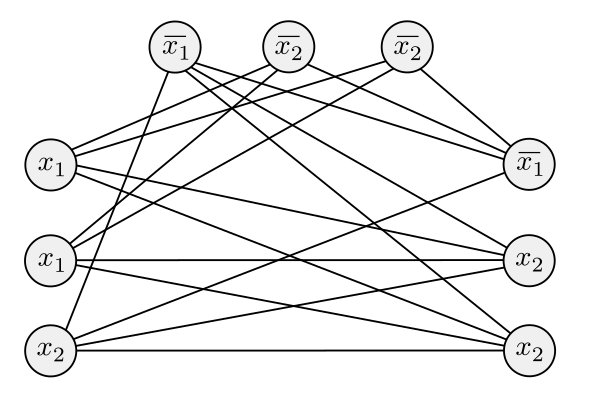
\includegraphics[scale=0.5]{figur/figur733.png}
		\item Husk at en $k$-klikke er en komplet delgraf af størrelse $k$ af en større graf $G$.
		\item Altså hvor alle knuderne er forbundet af kanter.
	\end{itemize}

	\begin{theorem}
		$\phi$  er satisfiable $\iff$ $G$ har en $k$-klikke.
	\end{theorem}

	\begin{itemize}
		\item Antag at $\phi$ har en satisfying tildeling.
		\item \(\Rightarrow\) Ved en sådan tiledeling er der mindst én literal i hver klausul der evalueres til at være sand. (Altså den evalueres til at være sand, Jørgen spurgte mig om dette i DM551 eksamen!)
		\item I hver triple i $G$ vælger vi en knude korresponderende til en sand literal i den tildeling der er satisfying.
		\item Hvis mere end én literal er sand vælger vi arbitrært en af dem.
		\item De knuder vi vælger giver en $k$-klikke.
		\item Antallet af knuder vi har valgt er $k$, fordi vi vælger en fra hver af de $k$ tripler.
		\item Det er en $k$-klikke fordi:
		      \begin{enumerate}
			      \item De kan ikke være fra samme triple, og dermed ikke have en kant mellem sig
			      \item De kan ikke være uoverensstemmelige, da de begge skal have en \textit{sand} sandhedsværdi.
		      \end{enumerate}
		\item \(\Leftarrow\) Antag at $G$ har en $k$-klikk. Ingen af de to knuder kan være i samme triple. Dermed må hver af de $k$ tripler have præcis én af knuderne.
		\item Vi tildeler sandhedsværdier til variablerne i $\phi$ så hver literal  der er en del af klikke knuderne bliver gjort sand.
		\item Dette er altid muligt da der ikke er kanter mellem uoverensstemmelige literale.
		\item Denne tildeling af sandhedsværdier er sand, da der er mindst én sand literal i hver triple (klausul).
		\item Dermed er $\phi$ satisfiable.
	\end{itemize}
\end{frame}

\begin{frame}[allowframebreaks]
	\frametitle{Definitionen af NP-Komplethed}
	\begin{definition}
		Et sprog $B$ er $NP$-komplet hvis det satisfier to betingelser:
		\begin{enumerate}
			\item $B \in NP$
			\item $\forall A \in NP : A \le_{P} B$
		\end{enumerate}
	\end{definition}

	\begin{theorem}
		Hvis $B$ er NP-Komplet og $B \in P$, så er $P = NP$.
	\end{theorem}

	\begin{itemize}
		\item Beviset følger fra definitionen af reducerbarhed i polynomiel tid.
	\end{itemize}

	\begin{theorem}
		Hvis $B$ er NP-Komplet og $B \le_{P} C$ for $C \in NP$ så er $C$ NP-komplet.
	\end{theorem}
	\begin{itemize}
		\item Vi ved allerede at $C \in NP$. Vi skal derfor vise at alle $A \in NP$ er reducerbart i polynomiel tid til $C$.
		\item Fordi $B$ er NP-Komplet, er hvert sprog i $NP$ reducerbart i polynomiel tid til $B$ og $B$ er polynomielt tid reducerbart til $C$.
		\item Hvis $A$ er polynomielt reducerbart til $B$  og $B$ til $C$, så er $A$ til $C$.
	\end{itemize}
\end{frame}

\begin{frame}[allowframebreaks]
	\frametitle{Vertex-Cover problemet}
	\begin{itemize}
		\item Ved en urettet graf $G$, er et \textit{vertex cover} af $G$ en delmængde af knuder hvor hver kant af $G$ rører en af disse knuder.
		      \begin{align*}
			      \text{VERTEX-COVER} & = \{\langle G , k \rangle \mid G \text{ er en urettet graf som har en } \\
			                          & k\text{-knude vertex cover.}\}
		      \end{align*}
	\end{itemize}
	\begin{theorem}
		VERTEX-COVER er NP-Komplet
	\end{theorem}

	\begin{itemize}
		\item Vi viser at 3-SAT er polytids reducerbart til VERTEX-COVER.
		\item Reduktionen konverterer en 3cnf-formel $\phi$ til en graf $G$ og et tal $k$, så $\phi$ er satisfiable når $G$ har et vertex cover med $k$ knuder.
		\item Til at bevise dette bruger vi ``gadgets'', som er små ``dele'', vi vil putte sammen.
		\item Vi kommer til at have to typer af disse ``gadgets'':
		      \begin{itemize}
			      \item Variabel Gadget: En lille graf for hver af variablerne
			      \item Klausul Gadget: En lille graf for hvert klausul
		      \end{itemize}

		\item Variabel gadgetten har to knuder. Givet en literal $v_{i}$, vil der være en knude $v_{i} \in V$  og $\overline{v_{i}} \in G$. Derudover vil $(v_{i}, \overline{v_{i}}) \in E$.
		\item At have denne variabel gadget skal sikre for os at vi kun vælger én af de knuder, fremfor begge.
		\item Givet en klausul $(v_{i} \lor v_{j} \lor v_{k})$ får vi en ``gadget'' hvor $\{v_{i}, v_{j}, v_{k}\} \in G$ og $\{(v_{i}, v_{k}), (v_{j}, v_{k}), (v_{j}, v_{i})\} \in E$. Altså får vi en form for trekant.
		\item Kort terminologi, $G_{V}$ er gadgateten der omhandler variabler og $G_{K}$ er gadgetten med klausuler. Derudover $G_{V} \cup G_{K} = G$
		\item Vi tilføjer nu kanter mellem alle knuder der har samme navn, så knuden $v_{i} \in G_{V}$ og knuden $v_{i} \in G_{K}$ skal have en kant mellem sig $(v_{i}, v_{i}) \in E$.
		\item Hvis en knude blive valgt til vertex-coveret, vil det betyde at sandhedsværdien skal være sand.
		\item Givet en formel $\phi$ der har $m$ variabler og $l$ klausuler, så har grafen $G = (V,E)$ antal knuder $|V| = 2m+3l$.
		\item Lad $k = m+2l$
		\item Følgende eksempel er for $\phi = (x_{1} \lor x_{1} \lor x_{2}) \land (\overline{x_{1}} \lor \overline{x_{2}} \lor \overline{x_{2}}) \land (\overline{x_{1}} \lor x_{2} \lor x_{2})$. For denne er $k = 8 = 2 + 2 \cdot 3$.
		      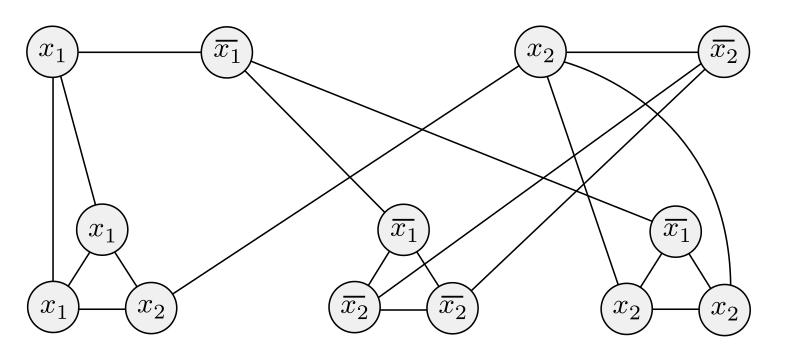
\includegraphics[scale=0.5]{figur/figur745.png}
		\item Grunden til at $k = m+2l$:
		      \begin{itemize}
			      \item $2l$ = Man skal vælge mindst 2 knuder for at cover hver kant
			      \item $m$ = Vi må kun vælge én af variablerne i variabel gadgetten.
		      \end{itemize}
		\item For at bevise at denne reduktion fungerer skal vi vise at:
		\item $\phi$ er satisfiable $\iff$ $G$ har et vertex cover med $k$ knuder.
		\item Hvis \(\phi\) er satisfiable \(\Rightarrow\) har $G$ et vertex cover med $k$ knuder.
		\item
	\end{itemize}
\end{frame}

%%% Local Variables:
%%% mode: latex
%%% TeX-engine: xetex
%%% TeX-command-extra-options: "-shell-escape"
%%% TeX-master: "main"
%%% End:
